% Multiple Choice Question 12 to 13 (2 questions)

\textbf{See the instruction for questions \inteval{\value{question}+1} to \inteval{\value{question}+2}.} 

\begin{center}
    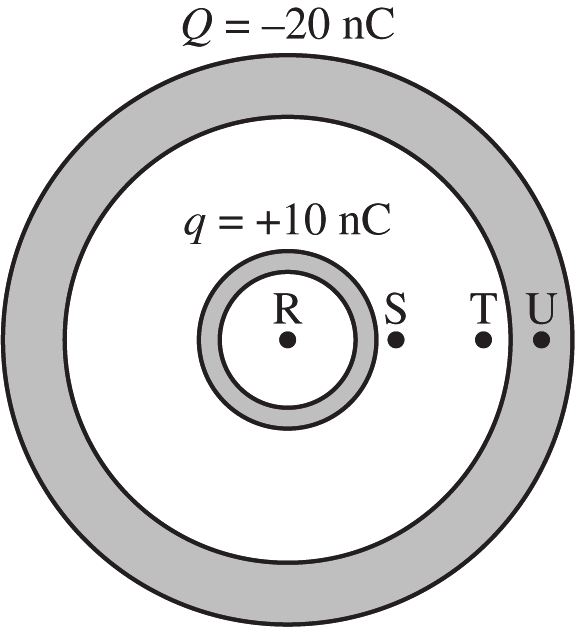
\includegraphics[scale=0.25]{images/img-007-007.png}
\end{center}

Two concentric spherical conducting shells and four labeled points are shown above. The outer shell has a net charge $Q=-20 \unit{nC}$. The inner shell has a net charge $q=+10 \unit{nC}$.

\begin{questions}
\setcounter{question}{11}

% Multiple Choice Question 12
\question
What is the charge on the outer surface of the outer shell?

\begin{oneparchoices}
    \choice $-30 \unit{nC}$
    \choice $-20 \unit{nC}$
    \choice $-10 \unit{nC}$
    \choice $+10 \unit{nC}$
    \choice $+30 \unit{nC}$
\end{oneparchoices}

% Multiple Choice Question 13
\question
The magnitudes of the electric fields at the four labeled points in the figure are $E_{\mathrm{R}}, E_{\mathrm{S}}, E_{\mathrm{T}}$, and $E_{\mathrm{U}}$, respectively. Which of the following correctly ranks the points according to the magnitude of their electric fields?

\begin{choices}
    \choice $E_{\mathrm{R}}=E_{\mathrm{S}}=E_{\mathrm{T}}=E_{\mathrm{U}}$
    \choice $E_{\mathrm{S}}>E_{\mathrm{T}}>\left(E_{\mathrm{R}}=E_{\mathrm{U}}\right)$
    \choice $\left(E_{\mathrm{S}}=E_{\mathrm{T}}\right)>E_{\mathrm{U}}>E_{\mathrm{R}}$
    \choice $E_{\mathrm{T}}>E_{\mathrm{S}}>E_{\mathrm{R}}>E_{\mathrm{U}}$
    \choice $\left(E_{\mathrm{S}}=E_{\mathrm{T}}\right)>\left(E_{\mathrm{R}}=E_{\mathrm{U}}\right)$
\end{choices}

\end{questions}
